%!TEX root = ../../thesis.tex

\section{History}
\label{sec:rc-history}

\subsection{Early Systems}
The history of building automated reading comprehension systems dates back to over forty years ago. In the 1970s, researchers already recognized the importance of reading comprehension as an appropriate way of testing the language understanding abilities of computer programs.

% \red{TODO: want to cite \cite{charniak1972toward} but I don't know much of its context.}

One of the most notable early works is the \sys{QUALM} system detailed in \newcite{lehnert1977process}. Built on top of the framework of scripts and plans as devices for modeling human story comprehension \cite{schank1977scripts}, \newcite{lehnert1977process} devised a theory of question answering and focused on pragmatic issues and the importance of the context of the story in responding to questions. This early work set a strong vision for language understanding, but the actual systems built at that time were very small and limited to hand-coded scripts, and difficult to generalize to broader domains.

Due to the complexity of the problem, this line of research was mostly neglected in the 1980s and 1990s.\footnote{There has been a large body of work in story comprehension developed within the psychology community, see \cite{kintsch1998comprehension}.} In the late 1990s, there was some small revival of interest, following the creation of a reading comprehension dataset by \newcite{hirschman1999deep} and a subsequent Workshop on Reading Comprehension Tests as Evaluation for Computer-based Understanding Systems at ANLP/NAACL 2000. The dataset consists of 60 stories for development and 60 stories for testing of 3rd to 6th grade material, followed by short-answer \ti{who}, \ti{what}, \ti{when}, \ti{where} and \ti{why} questions. It only requires systems to return a sentence which contains the right answer. The systems developed at this stage were mostly rule-based bag-of-words approaches with shallow linguistic processing such as stemming, semantic class identification and pronoun resolution in the \sys{Deep Read} system \cite{hirschman1999deep}, or manually generated rules based on lexical and semantic correspondence in the \sys{Quarc} system \cite{riloff2000rule} or their combinations \cite{charniak2000reading}. These systems achieved $30\%$--$40\%$ accuracy on retrieving the correct sentence.

% {\red{TODO: add a sentence about TREC QA?}}

\subsection{Machine Learning Approaches}
\label{sec:ml-approaches}

\afterpage{
\LTcapwidth=\textwidth
\begin{longtable}{l | p{13.5cm}}
\toprule
\text{(a)} & \tf{CNN/Daily Mail} (cloze style) \\
& \tf{passage}: {\small ( @entity4 ) if you feel a ripple in the force today , it may be the news that the official @entity6 is getting its first gay character . according to the sci-fi website @entity9 , the upcoming novel `` @entity11 '' will feature a capable but flawed @entity13 official named @entity14 who `` also happens to be a lesbian . '' the character is the first gay figure in the official @entity6 -- the movies , television shows , comics and books approved by @entity6 franchise owner @entity22 -- according to @entity24 , editor of `` @entity6 '' books at @entity28 imprint @entity26 .} \\
& \tf{question}: {\small characters in `` \underline{\hspace{1cm}} '' movies have gradually become more diverse} \\
& \tf{answer}: {\small @entity6} \\
\midrule
\text{(b)} & \tf{MCTest} (multiple choice) \\
& \tf{passage}: {\small Once upon a time, there was a cowgirl named Clementine. Orange was her favorite color. Her favorite food was the strawberry. She really liked her Blackberry phone, which allowed her to call her friends and family when out on the range. One day Clementine thought she needed a new pair of boots, so she went to the mall. Before Clementine went inside the mall, she smoked a cigarette. Then she got a new pair of boots. She couldn't choose between brown and red. Finally she chose red, which the seller really liked. Once she got home, she found that her red boots didn't match her blue cowgirl clothes, so she knew she needed to return them. She traded them for a brown pair. While she was there, she also bought a pretzel from Auntie Anne's.} \\
&\tf{question}: {\small What did the cowgirl do before buying new boots?} \\
&\tf{hypothesized answers}: {\small A. She ate an orange B. She ate a strawberry C. She called her friend D. She smoked a cigarette} \\
&\tf{answer}: {\small D. She smoked a cigarette} \\
\midrule
\text{(c)} &\tf{SQuAD} (span prediction) \\
&\tf{passage}: {\small Super Bowl 50 was an American football game to determine the champion of the National Football League (NFL) for the 2015 season. The American Football Conference (AFC) champion \hl{Denver Broncos} defeated the National Football Conference (NFC) champion Carolina Panthers 24–10 to earn their third Super Bowl title. The game was played on February 7, 2016, at Levi's Stadium in the San Francisco Bay Area at Santa Clara, California. As this was the 50th Super Bowl, the league emphasized the "golden anniversary" with various gold-themed initiatives, as well as temporarily suspending the tradition of naming each Super Bowl game with Roman numerals (under which the game would have been known as "Super Bowl L"), so that the logo could prominently feature the Arabic numerals 50.}  \\
&\tf{question}: {\small Which NFL team won Super Bowl 50?} \\
&\tf{answer}: {\small Denver Broncos} \\
\midrule
\text{(d)} &\tf{NarrativeQA} (free-form text) \\
&\tf{passage}: {\small \ldots In the eyes of the city, they are now considered frauds. Five years later, Ray owns an occult bookstore and works as an unpopular children s entertainer with Winston; Egon has returned to Columbia University to conduct experiments into human emotion; and Peter hosts a pseudo-psychic television show. Peter's former girlfriend Dana Barrett has had a son, Oscar, with a violinist whom she married then divorced when he received an offer to join the London Symphony Orchestra.\ldots }  \\
&\tf{question}: {\small How is Oscar related to Dana?} \\
&\tf{answer}: {\small He is her son} \\
\bottomrule
\longcaption{Examples from representative reading comprehension datasets}{\label{tab:rc-examples} A few examples from representative reading comprehension datasets: (a) \sys{CNN/Daily Mail}~\cite{hermann2015teaching}, (b) \sys{MCTest}~\cite{richardson2013mctest}, (c) \sys{SQuAD}~\cite{rajpurkar2016squad} and (d) \sys{NarrativeQA}~\cite{kovcisky2018narrativeqa}.}
\end{longtable}
}

Between 2013 and 2015, there were remarkable efforts of formulating reading comprehension as a \ti{supervised learning} problem: researchers collected human-labeled training examples in the form of (passage, question, answer) triples, with the hope that we can train statistical models which learn to map a passage and question pair into their corresponding answer: $f: (\text{passage}, \text{question}) \longrightarrow \text{answer}.$

Two notable datasets during this period are \sys{MCTest}~\cite{richardson2013mctest} and \sys{ProcessBank}~\cite{berant2014modeling}. \sys{MCTest} collects 660 fictional stories, with 4 multiple choice questions per story (each question comes with 4 hypothetical answers and one of them is correct) (Table~\ref{tab:rc-examples} (b)). \sys{ProcessBank} is designed to answer binary-choice questions in a paragraph describing a biological process and requires an understanding of the relations between entities and events in the process. The dataset comprises 585 questions spread over the 200 paragraphs.

In the original \sys{MCTest} paper, \newcite{richardson2013mctest} proposed several rule-based baselines without leveraging any training data. One is a heuristic sliding window approach, which measures the weighted word overlap/distance information between words in the question, the answer and the sliding window; the other is to run an off-the-shelf textual entailment system by converting each question-answer pair into a statement. This dataset later inspired a strand of machine learning models \cite{sachan2015learning,narasimhan2015machine,wang2015machine}. These models were mostly built on top of a simple max-margin learning framework with a rich set of hand-engineered linguistic features, including syntactic dependencies, semantic frames, coreference resolution, discourse relations and word embeddings. The performance was improved modestly from 63\% to around 70\% on the \sys{MC500} portion. On the \sys{ProcessBank} dataset, \newcite{berant2014modeling} proposed a statistical model which learns to predict the process structure first and then maps the question to formal queries that can be executed against the structure. Similarly, the model incorporates a large set of manual features,\footnote{See \href{https://nlp.stanford.edu/pubs/berant-srikumar-manning-emnlp14-supp.pdf}{https://nlp.stanford.edu/pubs/berant-srikumar-manning-emnlp14-supp.pdf}.} and eventually obtains 66.7\% accuracy on the binary classification task.

These machine learning models have achieved modest progress compared to earlier rule-based heuristic methods. However, their improvements are still rather limited and their weaknesses are summarized as follows:
\begin{itemize}
    \item
        These models relied heavily on existing linguistic tools such as dependency parsers and semantic role labeling (SRL) systems. However, these linguistic representation tasks are far from solved and off-the-shelf tools are often trained from one single domain (e.g., newswire articles) and suffer from generalization problems in practical use. Therefore, leveraging existing linguistic annotations as features sometimes adds noise in these feature-based machine learning models and the situation gets worse for higher level annotations (e.g., discourse relations vs. part-of-speech tagging).
    \item
        Simulating human-level comprehension is an elusive challenge and it is always the case that it is difficult to construct effective features from current linguistic representations. For example, for the third question in Figure~\ref{fig:mctest-example}: \ti{How many friends does Alyssa have in this story?}, it is impossible to construct an effective feature when the evidence is spread over the passage.
    \item
        Although it is inspiring that we can train models from human-labeled reading comprehension examples, these datasets are still too small to support expressive statistical models. For example, the English Penn Treebank dataset for training dependency parsers consists of 39,832 examples, while in \sys{MCTest}, only 1,480 examples are used for training --- let alone reading comprehension which, as a comprehensive language understanding task, is more complex and requires different reasoning capabilities.
\end{itemize}

\subsection{A Resurgence: The Deep Learning Era}
\label{sec:deep-learning-era}

A turning point for this field came in 2015. The DeepMind researchers \newcite{hermann2015teaching} proposed a novel and cheap solution for creating large-scale supervised training data for learning reading comprehension models. They also proposed a neural network model --- an attention-based LSTM model named \sys{The Attentive Reader} --- and demonstrated that it outperformed symbolic NLP approaches by a large margin. In their experiments, the \sys{Attentive Reader} achieved 63.8\% accuracy while symbolic NLP systems obtained 50.9\% at most on the \sys{CNN} dataset.  The idea of the data creation is as follows: CNN and Daily Mail are accompanied by a number of bullet points, summarizing aspects of the information contained in the article. They take a news article as the passage and convert one of its bullet points as a cloze style question by replacing one entity at at time with a placeholder, and the answer is this replaced entity. In order to ensure that systems approaching this task need to genuinely understand the passage, rather than using world knowledge or a language model to answer questions, they run entity recognition and coreference resolution systems and replace all the entity mentions in each coreference chain by an abstract entity marker e.g., \ti{@entity6} (see an example in Table~\ref{tab:rc-examples} (a)). As a result, nearly 1 million data examples were collected at almost no cost.

Taking a step further, our work \cite{chen2016thorough} investigated this first-ever large reading comprehension dataset and demonstrated that a simple, carefully designed neural network model (Section~\ref{sec:sar}) is able to push the performance to 72.4\% on the \sys{CNN} dataset, another 8.6\% absolute improvement. More importantly, we justified that the neural network models are better at recognizing lexical matches and paraphrases compared to conventional feature-based classifiers. However,  although this semi-synthetic dataset provides a promising avenue for training effective statistical models, we concluded that the dataset appears to be noisy due to its method of data creation and coreference errors and is limited for driving further progress.

To address these limitations, \newcite{rajpurkar2016squad} collected a new dataset named \sys{the Stanford Question Answering Dataset (SQuAD)}. The dataset contains 107,785 question-answer pairs on 536 Wikipedia articles and the questions were posed by crowdworkers, and the answer to every question is a span of text from the corresponding reading passage (Table~\ref{tab:rc-examples} (c)). \sys{SQuAD} was the first large-scale reading comprehension dataset with natural questions. Thanks to its high quality and reliable automatic evaluation, this dataset has spurred tremendous interest in the NLP community and become the central benchmark in this field. It in turn inspired a wide array of new reading comprehension models \cite{wang2017machine,seo2017bidirectional,chen2017reading,wang2017gated,yu2018qanet} and the progress has been rapid --- as of Oct 2018, the best-performing single system achieved an F1 score of 91.8\% \cite{devlin2018bert} which already exceeds the estimated human performance of 91.2\%, while a feature-based classifier built by the original authors in 2016 only obtained an F1 of 51.0\%, as shown in Figure~\ref{fig:squad-progress}.

\begin{figure}[!t]
\center
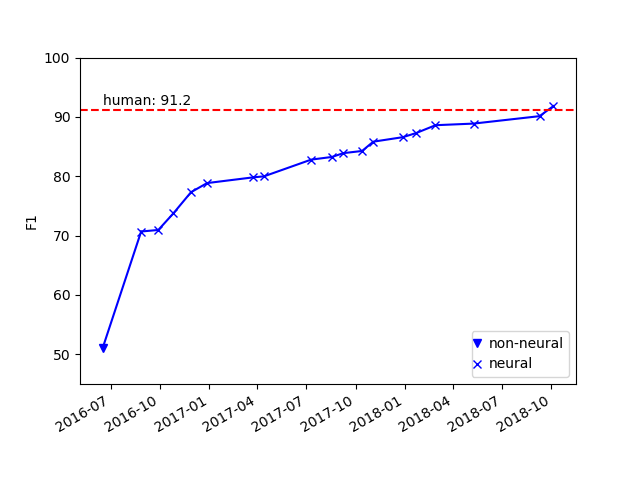
\includegraphics[scale=0.8]{img/squad_progress.png}
\longcaption{The progress on \sys{SQuAD} 1.1}{\label{fig:squad-progress}The progress on \sys{SQuAD} 1.1 (single model) since the dataset was released in June 2016. The data points are taken from the leaderboard at \href{http://stanford-qa.com/}{http://stanford-qa.com/}.}
\end{figure}

All the current top-performing systems on \sys{SQuAD} are built on \ti{end-to-end neural networks}, or \ti{deep learning} models. These models usually start off from the idea of representing every single word in the passage and question as a dense vector (e.g., 300 dimensions), passing through several modeling or interaction layers, and finally making predictions. All the parameters can be optimized jointly using the gradient descent algorithm or its variants. This class of models can be referred to as \ti{neural reading comprehension} and we will describe it in detail in Chapter~\ref{chapter:rc-models}. Differing from feature-based classifiers, neural reading comprehension models have several great advantages:
\begin{itemize}
    \item
        They don't rely on any downstream linguistic features (e.g., dependency parsing or coreference resolution) and all the features are learned on their own in one unified end-to-end framework. This can avoid noise in linguistic annotations while also providing great flexibility in the space of useful features.
    \item
        Conventional symbolic NLP systems suffer from one severe problem: features are usually very sparse and generalize poorly. For example, to answer a question ``\ti{How many individual libraries \tf{make up} the main school library?}'' from a passage ``\ldots\quad\quad\ti{Harvard Library, which is the world's largest academic and private library system, \tf{comprising} 79 individual libraries with over 18 million volumes.}'', a system has to learn the correspondence between \ti{comprising} and \ti{make up} based on indicator features such as:
        $$\text{pw}_i = \text{comprising} \wedge \text{qw}_{j} = \text{make} \wedge \text{qw}_{j + 1} = \text{up}.$$
        There is insufficient data to correctly weight most such features. It is a common problem in all non-neural NLP models. Making use of low-dimensional, dense word embeddings can effectively alleviate sparsity by sharing statistical strength between similar words.
    \item
        They are relieved from the labor of constructing a large set of manual features. Therefore, neural models are conceptually simpler and the focus can move to the design of neural architectures instead. Thanks to the development of modern deep learning frameworks such as \sys{Tensorflow} and \sys{PyTorch}, great progress has been made, and now it is fast and easy to develop new models.
\end{itemize}

% \red{TODO: add ``power of end-to-end optimization for a final goal''}
% \red{TODO: add ``more effective utilization of context in interpretation for WSD etc. This is what LSTMs give you!''}

There is no doubt that achieving human-performance on \sys{SQuAD} is incredible and arguably one of the biggest results we have seen in the NLP community in the past few years. Nevertheless, solving the \sys{SQuAD} task isn't equivalent to solving machine reading comprehension. We need to acknowledge that SQuAD is restricted in that questions must be answered using a single span in the passage and most SQuAD examples are fairly simple and don't really need complex reasoning.

The field has been further evolving. Following the theme of creating large-scale and more challenging reading comprehension datasets, a multitude of datasets have been collected recently: \sys{TriviaQA} \cite{joshi2017triviaqa}, \sys{RACE} \cite{lai2017race}, \sys{QAngaroo} \cite{welbl2018constructing}, \sys{NarrativeQA} \cite{kovcisky2018narrativeqa}, \sys{MultiRC} \cite{khashabi2018looking}, SQuAD 2.0~\cite{rajpurkar2018know}, \sys{HotpotQA}~\cite{yang2018hotpotqa} and many others. These datasets were collected from a variety of sources (Wikipedia, newswire articles, fictional stories or other Web resources) and constructed in very different ways and they aim to tackle many challenges that haven't been addressed before --- questions which are curated independent of the passages, questions which require multiple sentences or even multiple documents to answer, questions based on long documents like a full book, or questions which are not answerable from the passage. At the time of this writing, most of these datasets have not been solved yet and there remains a large gap between state-of-the-art methods and human performance levels. Reading comprehension has become one of the most active fields in NLP today and there are still many open questions to solve. We will discuss the recent development of reading comprehension datasets in more detail in Section~\ref{sec:future-datasets}.
